\chapter{Theoretical background and problem statement}
\label{chap:theoretical-background}

Project scheduling is the problem of deciding \emph{when} each activity of a
project should be executed so that all constraints are respected and a planning
objective, most often the total project duration, is optimised. In its
resource-constrained form the problem remains among the most intractable in
combinatorial optimisation~\cite{blazewicz1983,hartmann2010survey}, which is
precisely why \emph{evolutionary algorithms} continue to be one of the most
successful solution paradigms for it \cite{kolisch2006,khajesaeedi2025review}.
This thesis designs and evaluates such an algorithm for the multi-mode variant
of the problem. The present chapter establishes the necessary background:
Section \ref{sec:opt-pm} reviews how classical project management analyses and
optimises schedules through the \emph{critical path} and \emph{slack};
Section \ref{sec:challenges} explains why limited resources turn scheduling into
an NP-hard problem and why this favours evolutionary metaheuristics; and
Section~\ref{sec:problem-statement} states the concrete problem and the research
objectives of the thesis.

%==============================================================================
\section{Optimization in project management}
\label{sec:opt-pm}
%==============================================================================

A project is a temporary endeavour composed of a set of \emph{activities} (also
called tasks or jobs) linked by \emph{precedence relations}: an activity may
start only after all of its predecessors have finished~\cite{pmbok2021}. The two
foundational techniques for analysing such a project are the Critical Path
Method (CPM) and the Program Evaluation and Review Technique (PERT). Both
reduce a project to a directed acyclic
network and remain the analytical basis of modern project-management standards
and tools~\cite{pmbok2021} as well as the starting point of the research
literature on project scheduling \cite{demeulemeester2002}.

\subsection{The activity network and the critical path}
\label{subsec:cpm}

In the \emph{activity-on-node} (AoN) representation each activity $j$ is a node
with a fixed duration $d_j$, and a directed edge $(i,j)$ encodes the precedence
``$i$ must finish before $j$ starts''. Two dummy activities of zero duration, a
unique \emph{source} and a unique \emph{sink}, give the network a single entry
and exit point~\cite{demeulemeester2002}.

The \emph{critical path} is the longest chain of dependent activities through
the network, measured in time. Its length equals the shortest possible project
duration, the \emph{makespan}~$C_{\max}$, because the activities on this chain
must run one after another with no overlap. \changed{The notation $C_{\max}$ is the
standard one in the scheduling literature, going back to its
machine-scheduling roots~\cite{blazewicz1983} and used by the standard
notation review of Brucker et al.~\cite{brucker1999} as well as the
surveys and benchmark libraries this thesis builds
on~\cite{hartmann2010survey,vanpeteghem2014}: writing $C_j$ for the completion
time of activity $j$, the makespan is the completion time of the last
activity to finish, $C_{\max} = \max_j C_j$; the maximum is thus taken over
the activities of one schedule, not over possible schedules.} Activities on
the critical path are \emph{critical}: delaying any of them delays the whole
project.

\subsection{Forward and backward pass}
\label{subsec:passes}

For every activity CPM computes four time values: the \emph{earliest start
time} $EST_j$ and \emph{earliest finish time} $EFT_j$, and the \emph{latest
start time} $LST_j$ and \emph{latest finish time} $LFT_j$ that do not delay the
project~\cite{demeulemeester2002}.

\paragraph{Forward pass.}
Writing $P_j$ for the set of immediate predecessor activities of activity $j$,
and starting from the source at time $0$ and moving in topological order, the
earliest times are
\begin{align}
  EST_j &= \max_{\,i \,\in\, P_j} EFT_i,
         \qquad EST_{\text{source}} = 0, \label{eq:es}\\[2pt]
  EFT_j &= EST_j + d_j. \label{eq:ef}
\end{align}
Equation~\eqref{eq:es} states that an activity cannot start before \emph{all} of
its predecessors are finished, hence the maximum. The earliest finish of the
sink is the makespan, $C_{\max} = EFT_{\text{sink}}$.

\paragraph{Backward pass.}
Writing $S_j$ for the set of immediate successor activities of activity $j$,
and starting from the sink with $LFT_{\text{sink}} = C_{\max}$ and moving
against the edges, the latest times are
\begin{align}
  LFT_j &= \min_{\,i \,\in\, S_j} LST_i,
         \qquad LFT_{\text{sink}} = C_{\max}, \label{eq:lf}\\[2pt]
  LST_j &= LFT_j - d_j. \label{eq:ls}
\end{align}

\subsection{Slack: total float and free float}
\label{subsec:slack}

The \emph{slack} \changed{(also called \emph{float})} of an activity quantifies its scheduling
freedom. Two notions are distinguished~\cite{demeulemeester2002}. The
\emph{total float (total slack)} is the maximum delay from the earliest start
that does not delay project completion,
\begin{equation}
  TS_j = LST_j - EST_j = LFT_j - EFT_j, \label{eq:ts}
\end{equation}
the two forms being equal by~\eqref{eq:ef} and~\eqref{eq:ls}. The \emph{free
float (free slack)} is the maximum delay that does not delay the earliest
start of any successor,
\begin{equation}
  FS_j = \Big(\min_{\,i\,\in\,S_j} EST_i\Big) - EFT_j. \label{eq:fs}
\end{equation}
Since free float is measured against successors rather than the deadline,
$0 \le FS_j \le TS_j$ for every activity~\cite{demeulemeester2002}.

\subsection{A worked example}
\label{subsec:worked-example}

Consider a small project with six activities, with durations and precedence
relations given in Table~\ref{tab:example}. The corresponding activity-on-node
network with all four CPM time values and the total float is shown in
Figure~\ref{fig:cpm-network}.

\begin{table}[htbp]
  \centering
  \caption{Example project: durations and precedence relations.}
  \label{tab:example}
  \begin{tabular}{c c l}
    \toprule
    \textbf{Activity} & \textbf{Duration $d_j$} & \textbf{Predecessors} \\
    \midrule
    A & 3 & $-$  \\
    B & 4 & A    \\
    C & 2 & A    \\
    D & 5 & B, C \\
    E & 2 & C    \\
    F & 3 & D, E \\
    \bottomrule
  \end{tabular}
\end{table}

\begin{figure}[htbp]
  \centering
  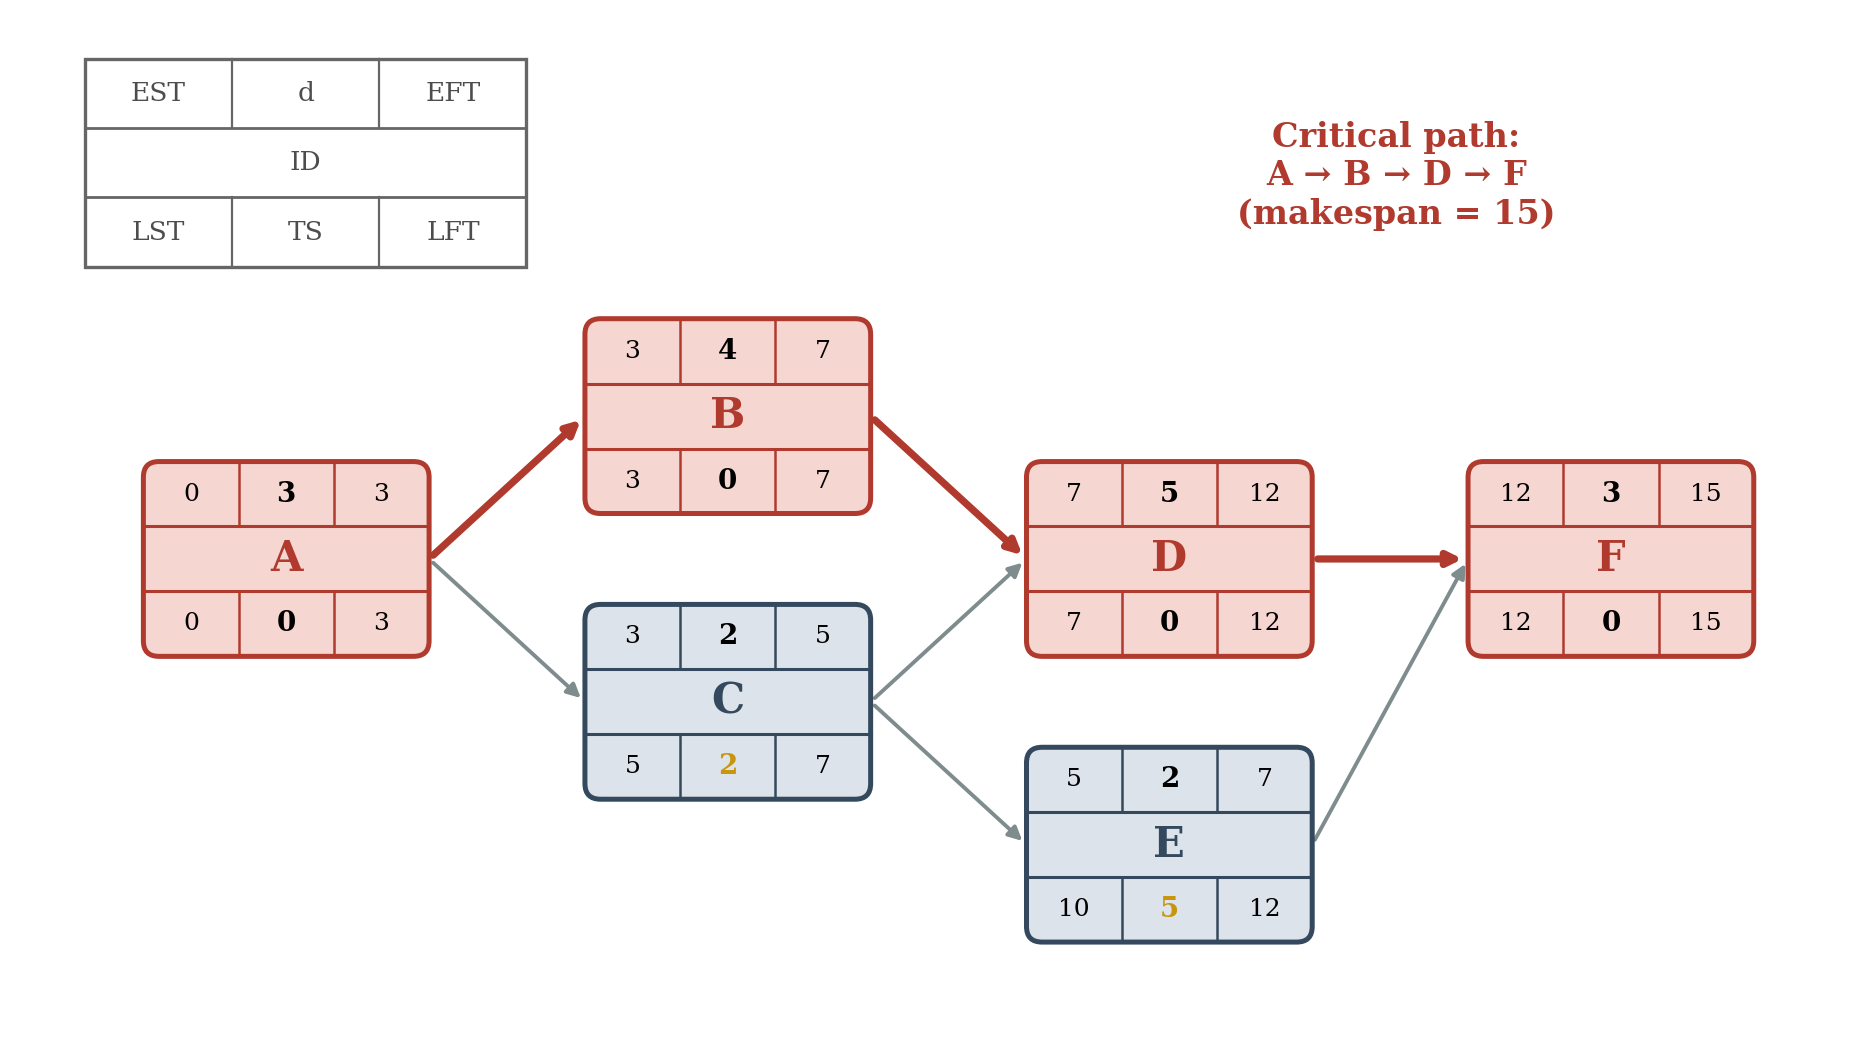
\includegraphics[width=\textwidth]{img/cpm-network.png}
  \caption[CPM activity-on-node network]{Activity-on-node network for the example
  of Table~\ref{tab:example}. Each node shows, from top to bottom,
  $(EST \mid d \mid EFT)$, the activity label, and $(LST \mid TS \mid LFT)$.
  Critical activities ($TS=0$) and the critical path
  $\text{A}\!\rightarrow\!\text{B}\!\rightarrow\!\text{D}\!\rightarrow\!\text{F}$
  are highlighted in red; the makespan is $C_{\max}=15$.}
  \label{fig:cpm-network}
\end{figure}

Applying the forward pass~\eqref{eq:es} and~\eqref{eq:ef} from the start gives
$EST_\text{A}=0,\ EFT_\text{A}=3$; then $EST_\text{B}=EST_\text{C}=EFT_\text{A}=3$, so
$EFT_\text{B}=7$ and $EFT_\text{C}=5$. Activity D waits for both B and C, hence
$EST_\text{D}=\max(EFT_\text{B},EFT_\text{C})=7$ and $EFT_\text{D}=12$. Finally
$EST_\text{F}=\max(EFT_\text{D},EFT_\text{E})=12$ and $EFT_\text{F}=15$, so the
makespan is $C_{\max}=15$.

The backward pass~\eqref{eq:lf} and~\eqref{eq:ls} starts from
$LFT_\text{F}=C_{\max}=15$ and propagates the latest times to the left. The
resulting slacks, from~\eqref{eq:ts}, are
$TS_\text{A}=TS_\text{B}=TS_\text{D}=TS_\text{F}=0$ (critical),
$TS_\text{C}=2$ and $TS_\text{E}=5$. The critical path is thus
$\text{A}\!\rightarrow\!\text{B}\!\rightarrow\!\text{D}\!\rightarrow\!\text{F}$.
Figure~\ref{fig:gantt-slack} renders the same schedule as a Gantt chart, with
each activity at its earliest start and the total float shown as a hatched
reserve to the right of the non-critical activities C and E.

\begin{figure}[htbp]
  \centering
  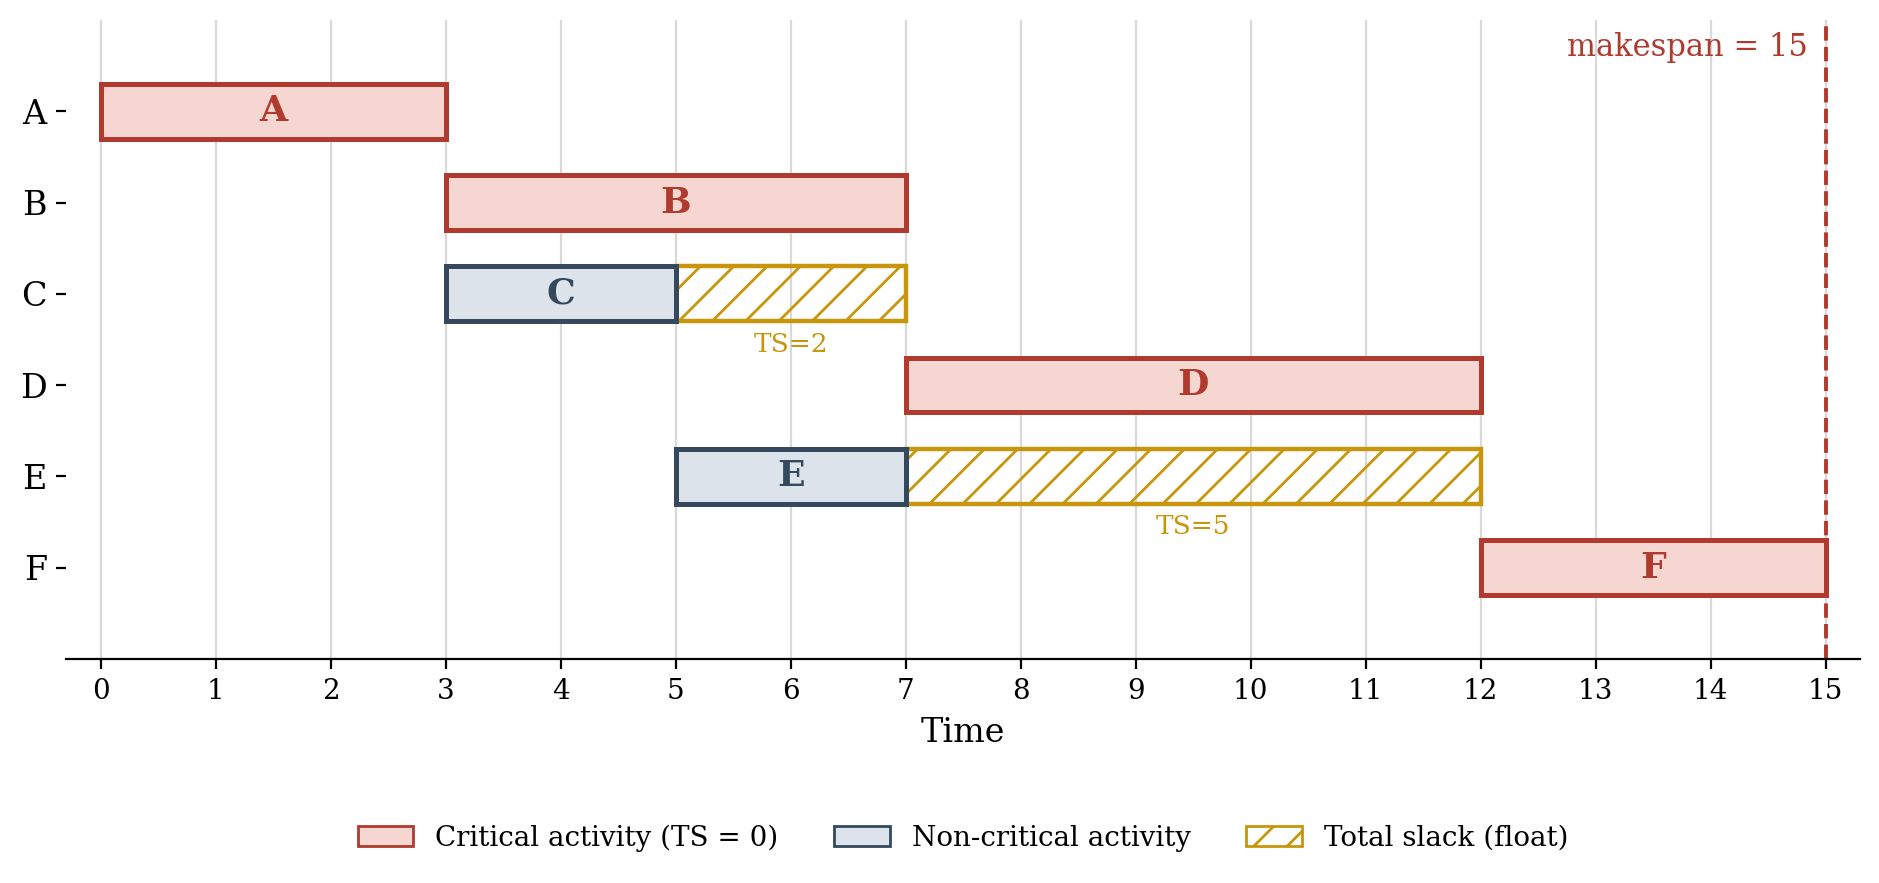
\includegraphics[width=\textwidth]{img/gantt-slack.png}
  \caption[Gantt chart with total float]{Early-start Gantt chart of the example
  project. Solid bars are activities at their earliest start; hatched bars show
  the total float (slack) of the non-critical activities C and E. Critical
  activities have no float and define the makespan $C_{\max}=15$.}
  \label{fig:gantt-slack}
\end{figure}

\subsection{Resource optimisation: levelling and smoothing}
\label{subsec:levelling-smoothing}

CPM as described so far assumes that resources are unlimited. In practice
activities compete for finite resources (people, machines, budget), and a
schedule that is feasible with respect to precedence may over-allocate a
resource~\cite{demeulemeester2002}. \emph{Resource
optimisation} adjusts the start dates of activities so that planned usage never
exceeds availability, and two complementary techniques are
distinguished~\cite{demeulemeester2002}. \emph{Resource levelling} is used when a
shared resource is over-allocated: it may move activities beyond their float,
typically by serialising parallel activities, so the resource limit, not the
precedence logic, drives the schedule. As a result levelling can change the
critical path and usually extends the project
duration~\cite{demeulemeester2002}. \emph{Resource
smoothing}, by contrast, adjusts activities only within their float, so the
critical path and the completion date are preserved while the resource profile
is flattened~\cite{demeulemeester2002}.

The crucial observation for this thesis is that as soon as resources are
limited, the simple longest-path computation of CPM no longer yields a feasible
schedule. Deciding \emph{which} activities to delay, and by how much, in order
to respect resource capacities while keeping the makespan small, is no longer a
polynomial network calculation but a hard combinatorial optimisation problem.
This is precisely the resource-constrained project scheduling problem studied in
the remainder of the thesis.

%==============================================================================
\section{Challenges in project scheduling}
\label{sec:challenges}
%==============================================================================

Adding resource constraints transforms project scheduling into the strongly \emph{NP-hard} Resource-Constrained Project Scheduling Problem (RCPSP)~\cite{blazewicz1983,ganian2020complexity}. The multi-mode extension (MRCPSP) studied here is even harder: once non-renewable resources are present, already \emph{deciding feasibility} (finding any mode assignment that respects the budgets) is NP-complete, as proved by Kolisch and Drexl~\cite{kolischdrexl1994} and confirmed in the recent complexity map of Ganian et al.~\cite{ganian2020complexity}.

This difficulty stems from a massive search space. In the MRCPSP, the exponentially growing combinations of valid start times are further multiplied by the available execution modes~\cite{kolischdrexl1994,hartmann2010survey}. Because exact methods like branch-and-bound can only solve small instances, evolutionary algorithms and other metaheuristics dominate larger applications~\cite{hartmann2002,kolisch2006,khajesaeedi2025review}.

Furthermore, constraints are tightly coupled: resolving a single resource conflict can cascade into new violations or alter the critical path~\cite{demeulemeester2002,khajesaeedi2025review}. Real-world scheduling also introduces conflicting multi-objective goals, such as project lead time versus resource-load balance~\cite{yang2024biobjective} or completion time versus cost~\cite{tian2022multiskill}, and parameter uncertainty~\cite{herroelen2005,ramos2023stochastic}. Standardised evaluation of these complexities relies on established benchmark libraries such as PSPLIB~\cite{kolisch1997} and the larger, multi-mode-specific MMLIB~\cite{vanpeteghem2014}; MMLIB50 and MMLIB100 (Section~\ref{subsec:mmlib}) are what this thesis's own empirical work is evaluated on.

Ultimately, these properties (an exponential, irregular search space, tightly coupled constraints, and the absence of exploitable global structure) make the MRCPSP exceptionally well-suited for population-based metaheuristics. \changed{Evolutionary algorithms require nothing of the problem beyond the ability to evaluate and compare candidate solutions, relying on selection and variation to navigate difficult landscapes. Given their strong empirical record on project scheduling specifically,} from the classic genetic algorithms of Hartmann~\cite{hartmann1998,hartmann2002} to systematic computational comparisons~\cite{kolisch2006,vanpeteghem2014} and recent surveys~\cite{khajesaeedi2025review,dokeroglu2025metaheuristics}, they form the foundation of the approach pursued in the remainder of this thesis.
%==============================================================================
\section{Problem statement and research objectives}
\label{sec:problem-statement}
%==============================================================================
\changed{This section states the target problem precisely
(Section~\ref{subsec:problem-statement}) and derives the research objectives
the thesis pursues (Section~\ref{subsec:objectives}).}
\subsection{Problem statement}
\label{subsec:problem-statement}

This thesis addresses the \emph{Multi-mode Resource-Constrained Project
Scheduling Problem} (MRCPSP)~\cite{brucker1999,hartmann2010survey}. We are given
a project of \emph{non-preemptive} activities \changed{(once started, an activity runs
to completion and cannot be interrupted)}
linked by precedence relations. Each activity may be executed in one of several
\emph{modes}; choosing a mode fixes the duration of the activity and the amounts
of the \emph{renewable} resources (e.g. labour or machines, available afresh each
period) and \emph{non-renewable} resources (e.g. a fixed budget, consumed over
the whole project) that it requires \cite{kolischdrexl1994,hartmann2010survey}.
A solution must select exactly one mode per
activity and a start time for every activity such that

\begin{enumerate}
  \item every activity starts only after all its predecessors have finished
        (precedence feasibility);
  \item at no point in time does the total demand for any renewable resource
        exceed its per-period availability;
  \item the total consumption of each non-renewable resource over the project
        does not exceed its budget.
\end{enumerate}

The objective is to minimise the project \emph{makespan} $C_{\max}$, the
completion time of the final activity, subject to the three constraint classes
above. This is the canonical objective in the benchmark
literature~\cite{kolisch1997,demeulemeester2002}; it reduces to the
single-mode RCPSP when each activity has one mode and to the pure CPM
longest-path problem of Section~\ref{subsec:cpm} when resources are unlimited.
\changed{For the complexity reasons established in Section~\ref{sec:challenges}, this
thesis approaches the problem with an evolutionary
algorithm~\cite{hartmann1998,kolisch2006,vanpeteghem2014,khajesaeedi2025review}.}
As the baseline against which the algorithm proposed in this thesis is compared,
we adopt the genetic-programming hyper-heuristic (GPHH) of
Tian, Mei and Zhang~\cite{Tian2024GPHH}, which learns scheduling rules for the
multi-mode problem and represents a recent, competitive evolutionary approach to
the MRCPSP. The publicly available reference implementation of this GPHH is used
directly as the empirical baseline throughout the experimental evaluation in
Chapter~\ref{chap:experiments}.

\changed{Despite this competitiveness, the baseline leaves several concrete
opportunities unaddressed, in the information it exposes to the evolved
rule, in how it selects parents, and in the absence of any refinement of
the schedules its rules produce. Section~\ref{subsec:research-gap}
substantiates these in full once the necessary formal background is in
place, and Chapter~\ref{chap:approach} targets them with three additive,
independently switchable modifications of the baseline, so that the
individual contribution of each can be isolated experimentally in
Chapter~\ref{chap:experiments}.}

\subsection{Formal definition of the single-mode RCPSP}
\label{subsec:rcpsp-model}

\changed{The informal statement above is now made precise, starting with
the single-mode special case.}
Let $V = \{0, 1, \dots, n, n+1\}$ be the set of activities of a project, where
activity $0$ is a dummy \emph{source} and activity $n+1$ a dummy \emph{sink},
both of zero duration; this is the same activity-on-node convention used
informally in Section~\ref{subsec:cpm}~\cite{demeulemeester2002}, with $n$ the
number of non-dummy activities. Precedence relations form a set of directed
edges $E \subseteq V \times V$, and each activity $j$ has a fixed duration
$d_j \ge 0$ ($d_0 = d_{n+1} = 0$). A set $\mathcal{R}^{\rho}$ of \emph{renewable}
resources is available with a constant per-period capacity $R^{\rho}_k$ for
each $k \in \mathcal{R}^{\rho}$; activity $j$ requires $r^{\rho}_{jk} \ge 0$ units of
resource $k$ for its entire duration. Writing
$A(f,t) = \{\, j \in V : f_j - d_j \le t < f_j \,\}$ for the set of activities
active at time $t$ under a schedule (finish-time vector) $f = (f_j)_{j \in V}$,
the single-mode RCPSP is
\begin{align}
  \text{minimise } \quad & C_{\max} = f_{n+1} \label{eq:rcpsp-obj}\\
  \text{subject to } \quad
  & f_i \le f_j - d_j, && \forall (i,j) \in E, \label{eq:rcpsp-prec}\\
  & \sum_{j \,\in\, A(f,t)} r^{\rho}_{jk} \le R^{\rho}_k, && \forall k \in \mathcal{R}^{\rho},\ \forall t \ge 0, \label{eq:rcpsp-res}\\
  & f_j \ge d_j, && \forall j \in V. \label{eq:rcpsp-nonneg}
\end{align}
Constraint~\eqref{eq:rcpsp-prec} is exactly the precedence relation used by the
forward pass of CPM (Section~\ref{subsec:passes}); constraint~\eqref{eq:rcpsp-res}
is new and couples activities that CPM treats independently. This formulation
follows the conceptual linear-programming model of Demeulemeester and
Herroelen~\cite{demeulemeester2002} for the decision variables $f_j$ and
duration $d_j$, and the resource-classification notation
$\mathcal{R}^\rho,\mathcal{R}^\nu,R^\rho_k$ of Brucker et
al.~\cite{brucker1999}, whose unifying notation for project scheduling this
thesis adopts for resource sets and availabilities throughout.
Without~\eqref{eq:rcpsp-res} the problem reduces to the
longest-path computation of Section~\ref{subsec:cpm}; with it, deciding even
feasibility in the multi-mode case becomes NP-complete, as already noted in
Section~\ref{sec:challenges}.

\subsection{Formal definition of the multi-mode RCPSP}
\label{subsec:mrcpsp-model}

The MRCPSP augments the model of
Section~\ref{subsec:rcpsp-model} with a finite set of execution \emph{modes}
$\mathcal{M}_i$ for every activity $i$ and a second resource class. Choosing mode
$m \in \mathcal{M}_i$ fixes the activity's duration $d_{im}$, its demand $r^{\rho}_{imk}$ for each
renewable resource $k \in \mathcal{R}^{\rho}$, and its consumption $r^{\nu}_{imk}$ of each
\emph{non-renewable} resource $k \in \mathcal{R}^{\nu}$, a resource with a single budget
$R^{\nu}_k$ for the whole project rather than a per-period
capacity~\cite{kolischdrexl1994,hartmann2010survey}. With mode-assignment
variables $m_i \in \mathcal{M}_i$ added to the finish-time variables $f_i$, the model
becomes
\begin{align}
  \text{minimise } \quad & C_{\max} = f_{n+1} \label{eq:mrcpsp-obj}\\
  \text{subject to } \quad
  & f_i \le f_j - d_{j m_j}, && \forall (i,j) \in E, \label{eq:mrcpsp-prec}\\
  & \sum_{j \,\in\, A(f,t)} r^{\rho}_{j m_j k} \le R^{\rho}_k, && \forall k \in \mathcal{R}^{\rho},\ \forall t \ge 0, \label{eq:mrcpsp-res}\\
  & \sum_{j \,\in\, V} r^{\nu}_{j m_j k} \le R^{\nu}_k, && \forall k \in \mathcal{R}^{\nu}, \label{eq:mrcpsp-nr}\\
  & m_j \in \mathcal{M}_j,\ f_j \ge d_{j m_j}, && \forall j \in V. \label{eq:mrcpsp-mode}
\end{align}
Constraint~\eqref{eq:mrcpsp-nr} is what distinguishes the MRCPSP from a simple
RCPSP with per-mode durations: because it sums over the \emph{entire} project
rather than over a time window, it can be \changed{checked} only after every mode has
been fixed, which is exactly why Kolisch and Drexl proved that even checking
feasibility of a mode assignment is NP-complete~\cite{kolischdrexl1994}.
Setting $|\mathcal{M}_i|=1$ for every activity recovers the single-mode
model~\eqref{eq:rcpsp-obj}--\eqref{eq:rcpsp-nonneg} exactly.
Early heuristics for this exact problem combined a hand-designed priority rule
for activity selection with a second, equally hand-designed rule for mode
selection~\cite{boctor1996new,kolisch1994priority,lova2006mrcpsp}.

\subsection{A taxonomy of realistic extensions}
\label{subsec:taxonomy}

The MRCPSP is itself one of several directions in which the basic RCPSP has been
extended to better match real projects~\cite{hartmann2010survey,mika2015mrcpsp}.
Figure~\ref{fig:rcpsp-taxonomy} situates it among the variants most discussed
in the recent literature:
\begin{description}
  \item[Generalized precedence relations (MRCPSP/max)] replace the simple
        finish-to-start relation of~\eqref{eq:mrcpsp-prec} with minimal and
        maximal time lags between any pair of activities, first formalised by
        Bartusch, M\"ohring and Radermacher~\cite{bartusch1988}; even feasibility
        is NP-hard under this extension~\cite{hartmann2010survey}.
  \item[Preemptive variants] allow an activity to be interrupted and resumed
        later, trading schedule flexibility for a more complex SGS that must
        track partially completed activities~\cite{vanpeteghem2010}.
  \item[Multi-skill RCPSP] replaces anonymous renewable resources with named
        workers who each master a subset of required skills, adding a
        many-to-one assignment problem on top of scheduling; Tian et
        al.~\cite{tian2022multiskill} formulate this jointly with mode and
        skill-switch decisions for the multi-objective case.
  \item[Stochastic and robust RCPSP] treat durations or resource availability as
        uncertain rather than fixed, an issue surveyed early by Herroelen and
        Leus~\cite{herroelen2005} and addressed for the multi-mode case by Ramos
        et al.~\cite{ramos2023stochastic} with a multi-start iterated local
        search over a stochastic-programming formulation.
  \item[Multi-objective RCPSP] optimises makespan jointly with a second
        criterion, e.g. cost or resource-load balance; Yang et
        al.~\cite{yang2024biobjective} combine NSGA-II with $Q$-learning for a
        bi-objective (lead time vs.\ resource-load balance) multi-mode
        multi-project variant.
  \item[Dynamic / disrupted RCPSP] reacts online to disruptions revealed during
        execution, e.g. resource breakdowns, rather than planning the whole
        project up front~\cite{cai2024rlgnn}; Ruhlusara\c{c} and \c{C}al{\i}\c{s}kan
        address the related dynamic multi-mode \emph{multi-project} setting with
        an MILP model minimising weighted earliness and tardiness, validated on
        a real furniture-manufacturing case~\cite{ruhlusarac2022dynamic}.
\end{description}

\begin{figure}[htbp]
  \centering
  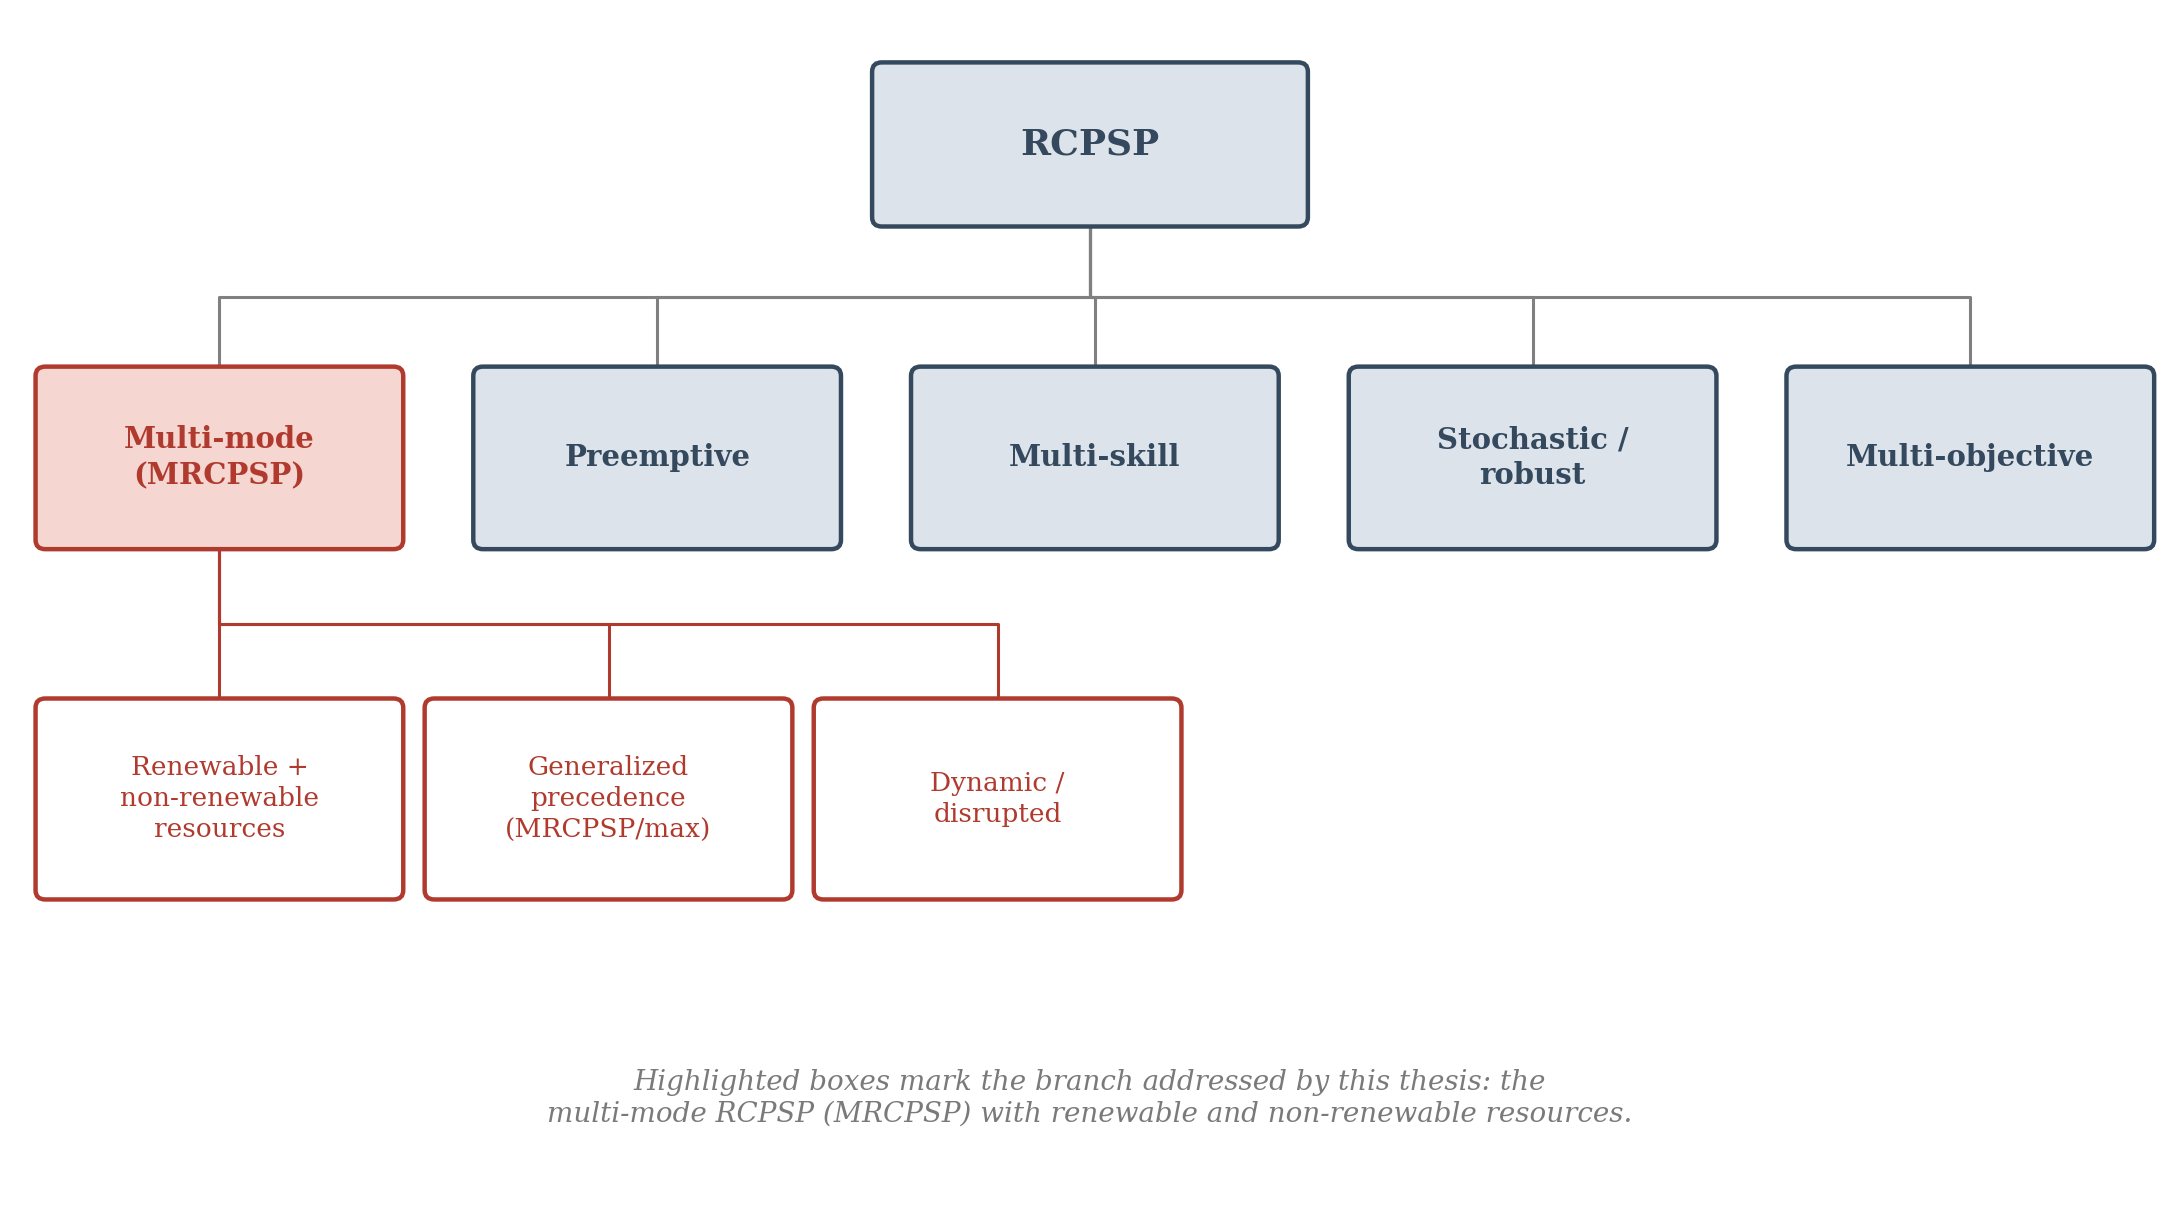
\includegraphics[width=0.92\textwidth]{img/rcpsp-taxonomy.png}
  \caption[Taxonomy of RCPSP extensions]{A taxonomy of realistic RCPSP
  extensions. This thesis addresses the multi-mode branch (MRCPSP) with both
  renewable and non-renewable resources (highlighted), the variant formalised
  in Section~\ref{subsec:mrcpsp-model}.}
  \label{fig:rcpsp-taxonomy}
\end{figure}

These extensions are not mutually exclusive (the multi-skill and
multi-objective variants above are themselves built on top of the multi-mode
model), which is why Hartmann and Briskorn's survey organises them as a
combinable feature set rather than a strict
hierarchy~\cite{hartmann2010survey}. Structural extensions beyond this
taxonomy also exist: van der Beek et al.~\cite{VanDerBeek2024} keep a single
makespan objective but relax which activities must even be executed (a
\emph{flexible project structure} in which only a subset of each ``selection
group'' need run) and allow non-renewable resources to be both consumed and
produced over the project, solving the resulting problem with a hybrid
differential-evolution algorithm, illustrating that real projects can
violate assumptions, such as a fixed activity set, that every variant above
still takes for granted. The present thesis keeps to the
``plain'' renewable-and-non-renewable MRCPSP of
Section~\ref{subsec:mrcpsp-model}, the variant for which the standard MMLIB and
PSPLIB benchmarks (Chapter~\ref{chap:dataset}) and the baseline algorithm of
Section~\ref{subsec:problem-statement} are defined.

\subsection{Research objectives}
\label{subsec:objectives}

The thesis pursues the following objectives:

\begin{enumerate}
  \item \textbf{Design.} To design a custom evolutionary algorithm for the
        MRCPSP.
  \item \textbf{Implementation.} To implement the algorithm in Python in a way
        that is reproducible and that can read the standard PSPLIB and MMLIB
        instance formats.
  \item \textbf{Analysis.} To analyse the behaviour of the algorithm 
        in order to understand which design choices
        contribute most to its performance.
  \item \textbf{Evaluation.} To evaluate the algorithm on the MMLIB50 and
        MMLIB100 benchmark sets~\cite{vanpeteghem2014} using standard
        quality metrics, and to compare it against our baseline, the
        genetic-programming hyper-heuristic of Tian, Mei and
        Zhang \cite{Tian2024GPHH}.
  \item \textbf{Discussion.} To discuss the computational complexity,
        scalability and limitations of the proposed approach, and to identify
        directions for future work.
\end{enumerate}
